\documentclass[11pt,a4paper]{article}
\usepackage[utf8]{inputenc}
\usepackage[a4paper]{geometry}

\usepackage[english]{babel}
\hyphenation{sil-la-ba-zio-ne pa-ren-te-si}
\usepackage{newlfont}

\usepackage{amsmath}
\usepackage{amsfonts}
\usepackage{amssymb}
\usepackage{amsthm}
\usepackage {amsmath, amssymb} 
\usepackage{bbm}

\usepackage{graphicx}
\usepackage{rotating}
\usepackage{subfigure}
\usepackage{lscape}
\usepackage[bf, scriptsize]{caption}
\usepackage{multirow}
\usepackage{longtable}
\hyphenation{Low-din}
\usepackage{titling}
\usepackage{eurosym}
\usepackage{adjustbox}

% included by Nicola for correct highlighting of C++ code
\usepackage{listings}
\usepackage{xcolor}

\definecolor{dkgreen}{rgb}{0,0.6,0}
\definecolor{dred}{rgb}{0.545,0,0}
\definecolor{dblue}{rgb}{0,0,0.545}
\definecolor{lgrey}{rgb}{0.9,0.9,0.9}
\definecolor{gray}{rgb}{0.4,0.4,0.4}
\definecolor{darkblue}{rgb}{0.0,0.0,0.6}

\lstdefinelanguage{cpp} {
      backgroundcolor=\color{lgrey},  
      basicstyle=\footnotesize \ttfamily \color{black} \bfseries,   
      breakatwhitespace=false,       
      breaklines=true,               
      captionpos=b,                   
      commentstyle=\color{dkgreen},   
      deletekeywords={...},          
      escapeinside={\%*} {*)},                  
      frame=single,                  
      language=C++,                
      keywordstyle=\color{purple},  
      morekeywords={BRIEFDescriptorConfig,string,TiXmlNode,DetectorDescriptorConfigContainer,istringstream,cerr,exit}, 
      identifierstyle=\color{black},
      stringstyle=\color{blue},      
      numbers=left,                 
      numbersep=5pt,                  
      numberstyle=\tiny\color{black}, 
      rulecolor=\color{black},        
      showspaces=false,               
      showstringspaces=false,        
      showtabs=false,                
      stepnumber=1,                   
      tabsize=2,                     
      title=\lstname,                 
    }
% end inclusion
\author{F. Cinus \& F. Delussu \& N. Sella}
\title{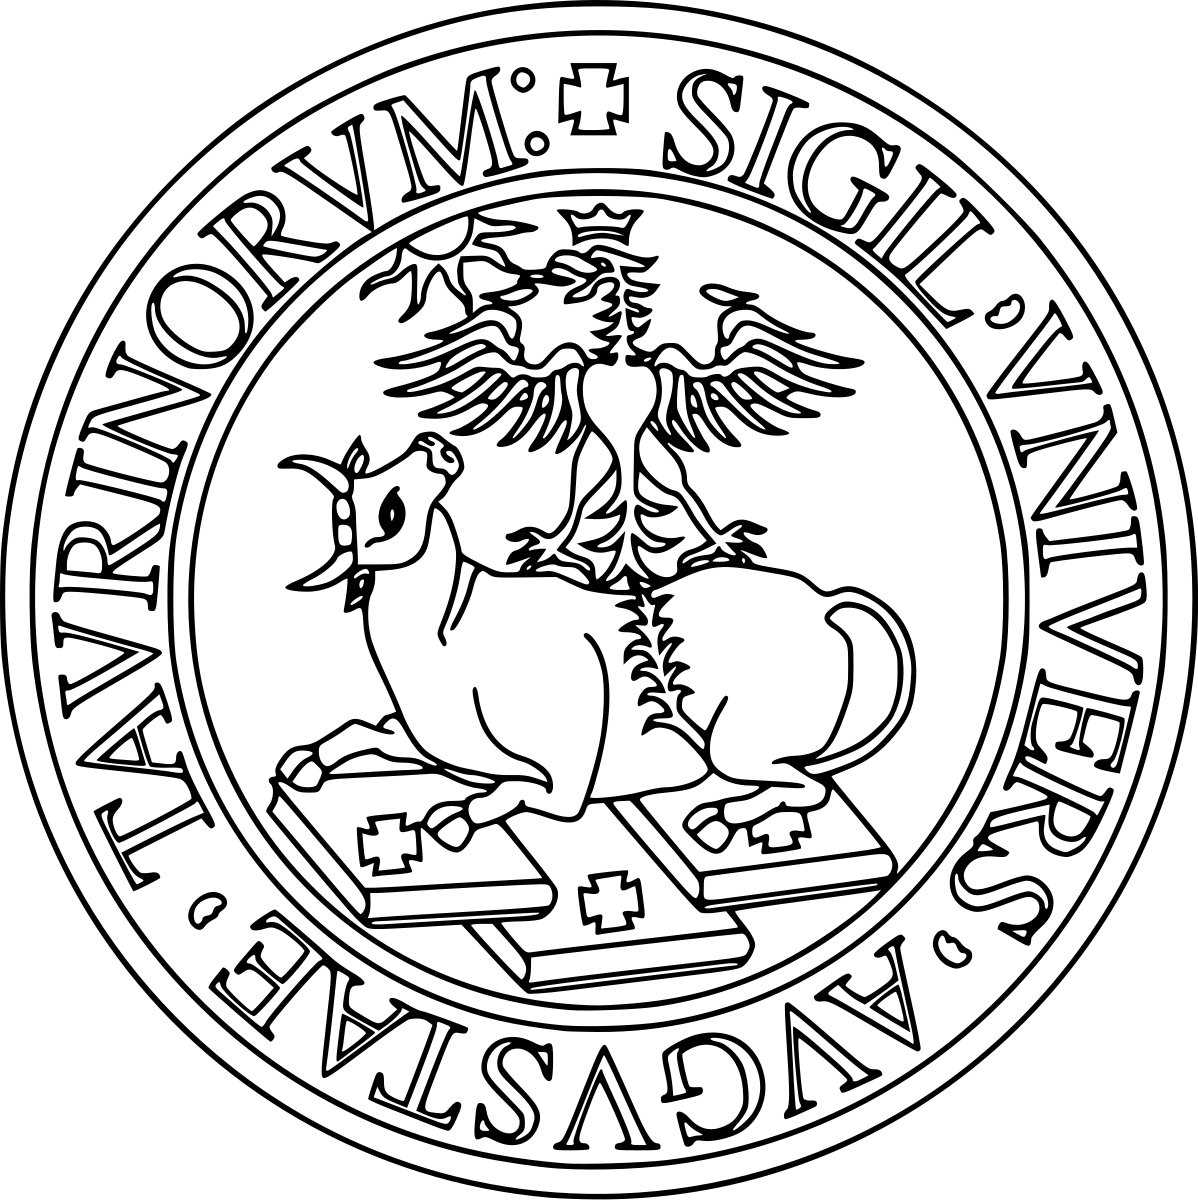
\includegraphics[scale=0.12]{Unito-logo} \\ \LARGE{UNIVERSIT\`{A} DEGLI STUDI DI TORINO} 
\\
TANS Course A.A. 2017/2018 Prof. Massimo Masera
\\
 \textbf{Ising Model Simulation with Monte Carlo methods}
}

\begin{document}
\date{}
\maketitle
\bigskip
\section*{Abstract}
In this work is introduced the Last Mile problem and the Agent-Based modelling process.
A solution for the Last Mile problem is proposed suggesting an active engagement of the population.
Some estimation has been done in order to make the simulation suitable for representing the city of Turin and actual cost of the delivering process.
Results show the robustness of the proposed solution both in economical and user's engagement terms, discussing also extreme situation.

%-----------------------------PAG 1----------------------------------%
\newpage
\section*{Introduction}
The Ising model is a well studied model in Statistical Mechanics which describes ferromagnetism phenomena. It is characterized by a microscopic configuration space based on D-dimensional lattice, that brings to macroscopic statistical quantities. Moreover it can easily generalize the concept of collective effects caused by binary valued points interacting in pairs; for this reason the Ising model became the core of the physics of complex systems. In the last decades computational methods have been applied to search a numerical solution for the 3D Ising model in order to  fill the lack of an analytical solution.  
\\
Alongside Metropolis algorithm became the most popular method of important sampling in MC. The basic idea of a weighted sampling based on the importance of a region determined a great step for the numerical solutions in general. Under these premises we want to outline the purpose this work wants to pursuit: finding numerical solution of the ND-dimensional Ising model with Metropolis algorithm.


\begin{figure}[h!]
\centering
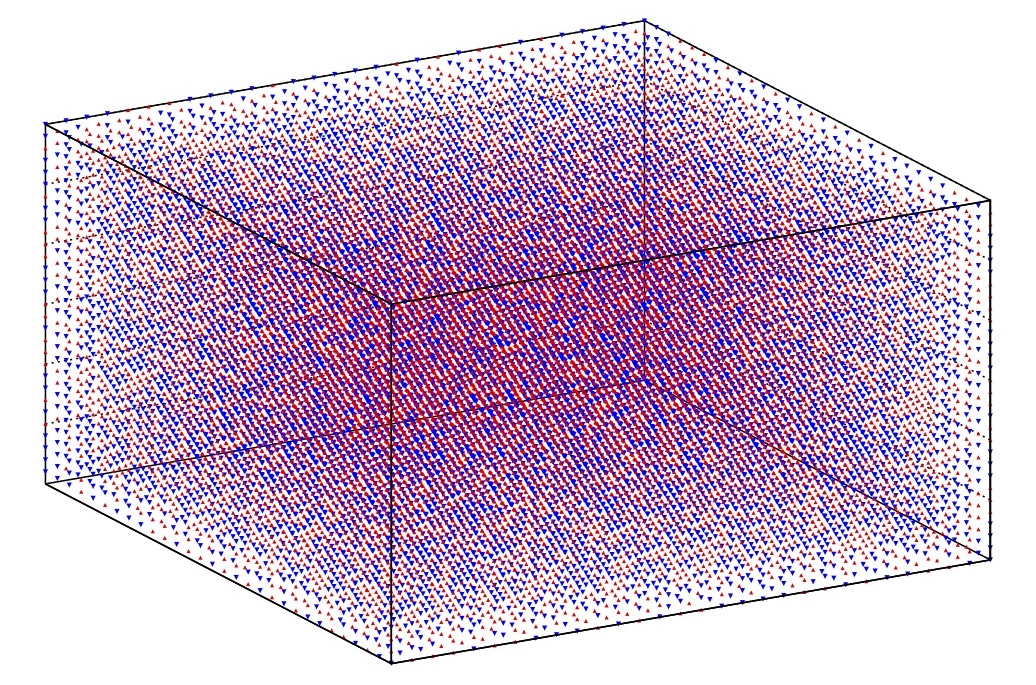
\includegraphics[scale=0.25]{img/img1_intro.jpg} 
\caption[Source: "monteinsing code" https://inknos.github.io/monteising/]{High temperature simulation of 3D Ising model}
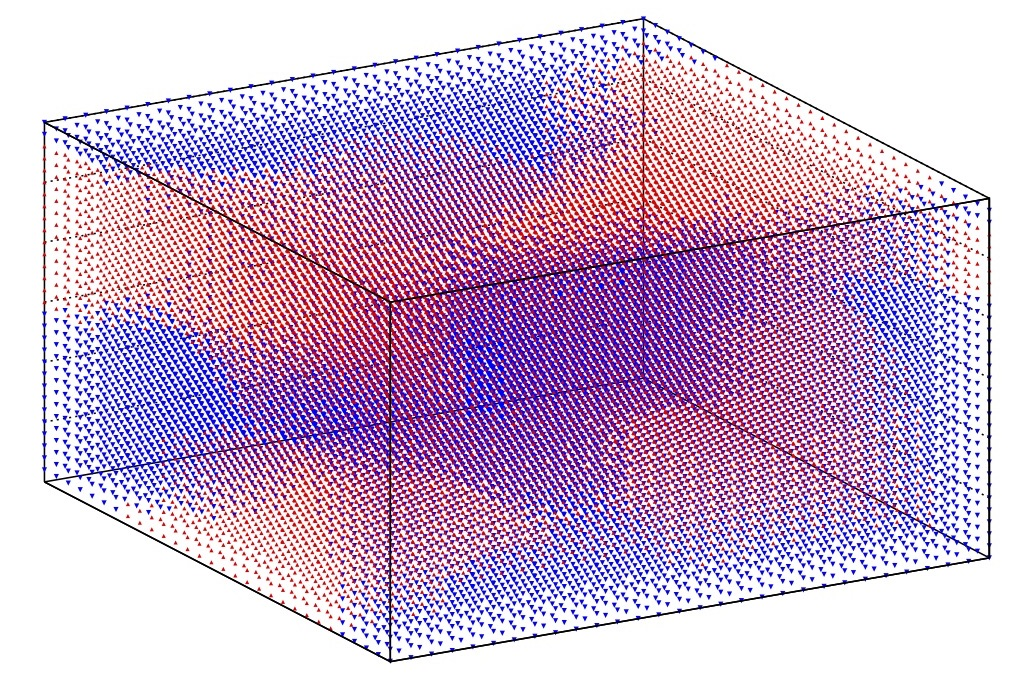
\includegraphics[scale=0.25]{img/img2_intro.jpg} 
\caption[Source: "monteinsing code" https://inknos.github.io/monteising/]{Low temperature simulation of 3D Ising model}
\end{figure}


%-----------------------------PAG 2----------------------------------%
\newpage 
\section{Theory}
\subsection{Ising model and importance sampling}
The Ising model is a physical-mathematical model characterized by a lattice of local spins in the [-1;+1] domain. The correspondent energy is proportional to the quadratic interaction of near spins ($\sigma_i$): 

\begin{equation}
H(q, \sigma) = \sum_{<l,m>}^{'} -J\sigma_i\sigma_j 
\end{equation}
Where $J$ is the energy interaction term and we sum over the neighbours.
\\
The system has  a macroscopic equilibrium state (macrostate) described by statistical quantities: number of spins $N$, lattice volume $V$, energy $E$, magnetization $M$. According to the Statistical Mechanics theory we consider the thermodynamic limit, i.e. $N, V \rightarrow \infty$ and $N/V = cost$ in order to have negligible fluctuations on energy and magnetisation: $(\Delta E)^2 / \langle E \rangle = O  (1/ \sqrt{N}) $.
From a theoretical point of view we consider an ensemble of lattices, each one with a particular configuration of spins (microstate) that corresponds to the same macrostate; we underlying that all microstates are equiprobable. The configuration space is described through the Hamiltonian formalism indeed, under ergodic hypothesis, the system visits all microstates. Moreover stationary hypothesis implies the existence of an equilibrium state in which  the probability distribution of the microstates satisfies the Liouville theorem. These hypotheses bring respectively to the following statements:

\begin{enumerate}
\item In the $t \rightarrow \infty$ limit: the average (over all the ensemble) of a physical quantity is equal to the temporal average of that quantity.
\item The probability distribution of the microstates depends only on the Hamiltonian:
\begin{equation}
\rho (q, \sigma ) \propto \exp \lbrace- \beta H(q, \sigma ) \rbrace 
\end{equation}
Where $q$ is the spin position on the lattice and $\beta$ is the product of the Boltzmann constant and the temperature $T$ of the system.
\end{enumerate}


In a finite case the Ising model system is characterized by magnetization and  energy fluctuations that brings us to consider it under canonical formalism. We define the partition function as follow: $Z = \sum_q exp [  -\beta H(q) ]$. The model simulation can be done through Monte Carlo method, i.e. we generate a pseudo-random chain of numbers in order to extract a microstate sample (from all the configuration space) distributed by the following equilibrium distribution of probability:
\begin{equation}
P_{eq}(q)=\exp \lbrace -\beta H(q)\rbrace /Z
\end{equation} 
In practice we cannot compute the partition function, moreover an algorithm that search over all the phase space has not a great performance. 


%-----------------------------PAG 3----------------------------------%
\newpage
The Boltzmann's factor as probability of choosing a configuration gives a great improvement for the simulation. In this way we are not sampling all the configuration space but a selected and uniform distributed microstates collection. This approach is called \textit{importance sampling} and it allows us to calculate physical quantities as the average number over the extracted configuration:
\begin{equation}
\langle E \rangle_N = \dfrac{1}{N} \sum_{i=1}^{N}{E(q_i)}
\end{equation} This intuition can be proved under ergodic hypothesis: in fact we can consider an evolving Ising system in which there is a spin flip at each time step. The temporal collection of microstates is a Markov chain with a transition probability ($W$) that leads the system to the equilibrium probability in the $t \rightarrow \infty$ limit. Indeed the ratio of the transition probability is:
$$ \dfrac{W(q \rightarrow q')}{W(q' \rightarrow q)} = \dfrac{P_{eq}(q')}{P_{eq}(q)}= \exp \lbrace \beta [E(q) - E(q')] \rbrace $$
Where $q$ and $q'$ are respectively the configuration before the spin-flip and after. This implies the equivalence between importance sampling and random extraction. The arbitrary choose on $W(q \rightarrow q')$ determines the particular algorithm; for the Metropolis-Hastings algorithm:

\begin{eqnarray}
W(q \rightarrow q')=1 \qquad \Delta E \leq 0 \\
W(q \rightarrow q')=\exp \lbrace -\beta \Delta E  \rbrace  \: \Delta E > 0
\end{eqnarray}

\bigskip

\subsection*{Phase transition in Ising model}
Magnetization in Ising model shows phase transition at a certain temperature called $T_c$. This means that the logarithm of the partition function has critical point of the first order in this point and two different statistical descriptions concurrently exist at $T_c$. Indeed the magnetization curve has two different fits before this point and after, that corresponds to inner configuration of spins: random that corresponds to $\langle M \rangle = 0$ and ordered with $\langle M \rangle \rightarrow +1 / -1$. 

 



%-----------------------------PAG 4----------------------------------%
\newpage 
\section{Code}
This section's aim is to introduce the reader to the C++ implementation of the model. The code is based on TObject class of Root and its scheme is the following:

\begin{figure}[h!]
\centering
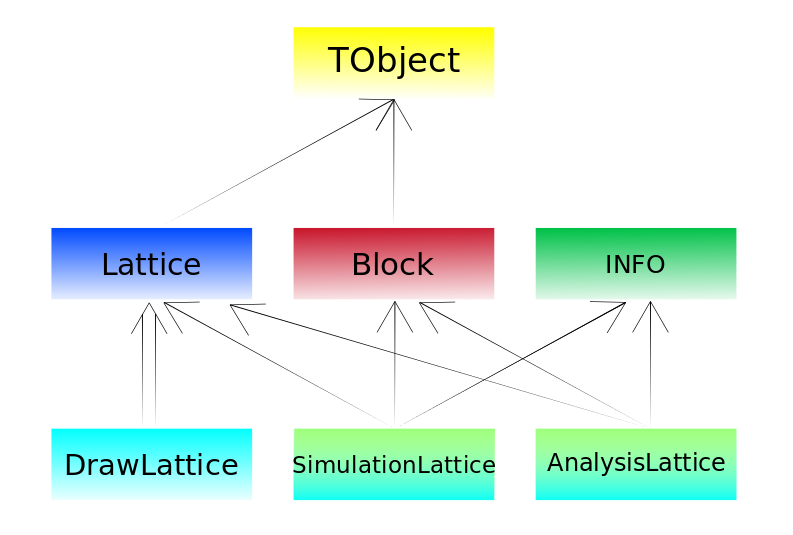
\includegraphics[scale=0.45]{img/Schema_classi.png}   
\caption{Class scheme}
\end{figure}




\subsection{Lattice Description}

The “lattice” array of a D-dimensional cubic Lattice is $\mathbf{L} = (L_0,L_1,..,L_{N^D-1})$.
Let $i$ denote the index of the array, ranging from $0$ to $N^D-1$.\\
Let $i$-$spin$ denote the spin represented by the $L_i$ boolean entry. \\
The cartesian coordinates $\mathbf{a} = (a_0,a_1,..,a_{D-1})$ of the $i$-spin can be computed from index $i$ if a convention is set on the lattice arrangement, which in our model is the following: 
\begin{itemize}
	\item The origin \textit{O} of the D-dimensional space is chosen to be a spin-vertex of the cubic Lattice such that each edge starting from \textit{O} is aligned along one of the D positive directions of the space. 
	\item The distance between each couple of adjacent spins is set to one. 
	\item The spins are indexed starting from increasing the first dimension’s coordinate, than the second and so forth.
\end{itemize}

%FIGURA caso 1 , 2 , 3 dimensionale

\textbf{N.B.} This rules imply that, given a specific spin, each coordinate $a_j$ takes values in range 
$\{0,1,…,N-1\}$. \\ 



%-----------------------------PAG 5----------------------------------%
\newpage


\subsection*{Coordinates Computation}

Cases from \textit{D=1} to \textit{D=3} are treated in order to understand and generalize the coordinates’ computation. \\
Before starting, the division $/$ and modulo $\%$ operators are defined as follows : \\
Given two integer numbers a and n , the operations a/n and a\%n return respectively the quotient and the remainder of the euclidean division of a by n. \\ 
\textit{e.g.} : $6/3=2$ ; $9/4=2$ ; $6\%3=0$ ; $9\%4=1$ \\

\vspace{0.1cm} 
\textbf{D=1} \\
A 1-dimensional lattice is made by $N$ spins aligned along a single $x$ direction .
In this case the index $i$ represents itself the $x$ coordinate of the spin.\\
%image 1D

\textbf{D=2} \\
A 2-dimensional Lattice is a square made by $N^2$ spins.\\
The index can be expressed as $i = a_0 + a_1N$. \\
$a_1$ can be seen as the number of $N$-spin lines stacked starting from the quote $y=0$, this number is
the $y$-cordinate itself while the number or remaining spin $a_0$ is the $x$-coordinate. 
$a_1$ is computed from $i$ divided by $N$ while $a_0$ is computed from $i$ modulo $N$.
The $(x,y)$ coordinates of the $i$-spin are given by : $$(a_0,a_1)=(i\%N ; i/N)$$ 


\textbf{D=3} \\
A 3-dimensional Lattice is a cube made by $N^{3}$ spins. \\  
The index $i$ can be expressed as $i = a_0 + a_1N + a_2N^2$. \\
$a_2$ can be seen as the number of $N^2$-spin squares stacked starting from the plane $z=0$, this number is 
the $z$ coordinate itself. $a_2$ is computed from $i/N$.
Once we have $a_2$ the remaining $(x,y)$ coordinates can be computed from \\ $i\%N^2 = a_0 + a_1N$ as in \{D=2\} case .\\
The $(x,y,z)$ coordinates of the $i$-spin are given by : $$(a_0,a_1,a_2)=\left( (i\%N^2)\%N , (i\%N^2)/N , i/N^2 \right)$$ 

Generalizing to $D$ dimensions, index $i$ can be expressed as :$ i = \sum_{j=1}^{D-1}a_jN^j $ \\
Its corresponding coordinates are computed starting from $j=D-1$ and establishing a recurrence relationship :
$$\mathbf{a} = \left(a_0 = i\%N ,.., a_j = [i\%N^{j+1}]/N^j ,.., a_{D-2} = [i\% N^{D-1}]/N^{D-2} , a_{D-1} = i/N^{D-1}\right)$$ 
 
%-----------------------------PAG 6----------------------------------%
 
\newpage
\subsection*{Lattice's energy } 

The Lattice's energy is computed according to equation (1).


%J is a constant interaction term between each couple $<l,m>$ of spins .\\
%The summation is performed over all possible couples $<l,m>$ of adjacent %spins.\\

The Lattice class provides a method wich returns the energy of the system. \\
The method's implemented algorithm takes the lattice array and performs two for loops, one over the system's dimension $d = (0,1,..,D-1)$ and the other over the lattice array's index $i = (0,1,..,N^D-1)$. \\
The key idea is that, given a fixed $i$-spin, along each dimension $d$ two neighbours $i_{d_\pm}$-spin are found on the increasing and decreasing d-coordinate respectively. 
\\So each single spin has $2D$ interacting neighbours in total, by summing up their energy interaction terms the contribute of the single spin to the total energy is obtained. So the energy can be rewritten as : 

$$H = \frac{1}{2}\sum_{i=0}^{N^D-1}\sum_{d=0}^{D-1}\sum_{\pm}^{} -J\sigma_i\sigma_{i_{d_\pm}}$$ 

It's easy to observe that, performing the first summation $\sum_{i}^{}$ , double countings of couples occur and a factor $1/2$ is required. \\ 
For each fixed index $i$ ,the algorithm takes into account only the interaction term with the 
$i_{d_+}$-spin so that the number of operation is halved. So the algorithm performs the summation :
  
$$H = \sum_{i=0}^{N^D-1}\sum_{d=0}^{D-1}-J(L_i \ \hat{} \ L_{i_{d_+}})$$ 

$\sigma_i\sigma_{i_{d_+}}$ has been replaced by $L_i \ \hat{} \ L_{i_{d_+}}$ , the former can take values $\pm1$ wether the two spins are aligned or not. Since spins are represented by boolean entries of array $\mathbf{L}$, the XOR bitwise operator $\hat{}$ is applied on couple $(L_i,L_{i_{d_+}})$ so that it returns the same value of $\sigma_i\sigma_{i_{d_+}}$. \\   
\vspace{0.1cm}
From the $i$ index coordinates $\mathbf{a} = (a_0,a_1,..,a_{D-1})$ the $i_{d_+}$ index coordinates 
$\mathbf{a^{d_+}} = (a^{d_+}_0,a^{d_+}_1,..,a^{d_+}_{D-1})$ can be computed. \\
The vector $\mathbf{a^{d_+}}$ differs from $\mathbf{a}$
only on the $d\deg$ entry $a^{d_+}_d$ which is the only one to be increased, this is computed as $(a_d+1)\%N$ since we are applying periodic boundary conditions on the Lattice. 

From this formulas we can express the $i_{d_+}$ index as the sum of two terms:
\begin{eqnarray*}
i_{d_+} &=& \left\{ \sum_{j = 0}^{d-1}a_jN^j  [(a_d + 1)\%N]N^d \right\} + \left\{ \sum_{j = d+1}^{D-1}a_jN^j \right\}  \\
&=& \left\{(i + N^d)\%N^{d+1} \right\}  +  \left\{ (i/N^{d+1})N^{d+1}  \right\} 
\end{eqnarray*}

The algorithm defines two powers \textsf{pow\textunderscore tmp1} and \textsf{pow\textunderscore tmp2}, keeping a fixed index $i$ and performing the loop over d, these powers are assigned respectively to $N^d$ and $N^{d+1}$ in each iteration.

\newpage 


\section*{Classes}
	
\subsection*{Lattice}

The Lattice class permits to construct a Lattice, compute its termodynamic quantities 
and change its state with the Metropolis Algorithm. \\	  
Computation details of functions such as \textbf{energy}() and \textbf{cooling}() are thoroughly explained in Model section. \\ 

\begin{itemize}

	\item[] 
	PRIVATE DATA MEMBERS \\ 
	
	\begin{tabular}{lll}
		const uint 		& \textbf{N}        & number of spins along one edge				  \\
		const uint 		& \textbf{dim}      & dimension										   \\
  		const uint 		& \textbf{num\textunderscore spin} & total number of spins : $N^{dim}$  \\
  		bool ${}^*$  	& \textbf{lattice}  & boolean array of size \textbf{num\textunderscore spin} \\
  		static double 	& \textbf{T}        & temperature  										  	  \\
	\end{tabular}
	\\

	\item[] 
	PUBLIC MEMBER FUNCTIONS \\ 
	\begin{itemize}
		\item[] CONSTRUCTORS \\

			\item[] \textbf{Lattice}()	 
			\begin{itemize}
				\item[] Default Constructor \\ 
						Creates Lattice object with N=1 , dim=1 \\
						The single entry of \textbf{lattice} is set to 0 or 1 with 0.5 probability   
			\end{itemize}
			
			\item[] \textbf{Lattice}(const uint\& \textunderscore N , const uint\& \textunderscore dim)	 
			\begin{itemize}
				\item[] Standard Constructor \\
						Creates Lattice object with N = \textunderscore N,  dim = \textunderscore dim \\
						Sets each \textbf{lattice} entry to 0 or 1 with 0.5 probability 
			\end{itemize}
			
			\item[] \textbf{Lattice}(const Lattice\& obj)		 
			\begin{itemize}
				\item[] Copy Constructor \\
						Creates Lattice object with obj's data members \\
			\end{itemize}

		
		\item[]
		DESTRUCTOR \\
		
			\item[] \textbf{$\sim$ Lattice}	 
			\begin{itemize}
				\item[] Frees up memory allocated by \textbf{lattice} \\
			\end{itemize}		
		
\newpage 		
	
		\item[] 
		PHYSICAL AND NUMERICAL FUNCTIONS \\
 		
			\item[] bool \textbf{flipSpin}(const uint\& n)		 
			\begin{itemize}
				\item[] If n $<$ \textbf{num\textunderscore spin} \\
				Sets \textbf{lattice}[n] to !\textbf{lattice}[n] and returns true \\
				Else it doesn't change \textbf{lattice} and returns false 
						
			\end{itemize}

			\item[] int \textbf{dE}(const uint\& n) const		 
			\begin{itemize}
				\item[] Returns energy variation resulting from applying \textbf{flipSpin}(n) \\
						{\small
						\textsf{n.b.} : it's a const method, it doesn't apply \textbf{flipSpin}(n)
						} 
			\end{itemize}
			
			\item[] int \textbf{energy}() const;		 
			\begin{itemize}
				\item[] Returns total Energy 
			\end{itemize} 
			
			\item[] float \textbf{magnetization}() const		 
			\begin{itemize}
				\item[] Returns Magnetization per site  
				
			\end{itemize}
			
			\item[] void \textbf{cooling}(const uint\& iter) 		 
			\begin{itemize}
				\item[] Applies one step of Metropolis Algorithm 
			\end{itemize}
			
			
			\item[] void \textbf{cooling}(const uint\& iter) 		 
			\begin{itemize}
				\item[] Applies \textbf{iter} steps of Metropolis Algorithm
			\end{itemize}
			
			\item[] double * \textbf{coolingPar}()	 
			\begin{itemize}
				\item[] Applies \textbf{cooling}() and returns a four-dimensional array \textbf{arr} \\
						\textbf{arr} are respectively variations of : \\
						Temperature , Energy , Magnetization , Energy per site  \\
			\end{itemize}
		
		\item[] 
		OVERLOADED OPERATORS \\

			\item[] Lattice\& \textbf{operator=}(const Lattice\& obj)		 
			\begin{itemize}
				\item[] Assignment operator \\
			\end{itemize}
			
			\item[] friend std::ostream\& \textbf{operator$<<$}(std::ostream\& out, const Lattice\& lat) 	
			\begin{itemize}
				\item[] Taking \textsf{lat} as a reference to a Lattice object \\
				Prints \textbf{lattice} member of \textsf{lat} by typing the command \textsf{cout $<<$ lat ;} 
			\end{itemize}	
			
			\item[] bool \textbf{operator==}(const Lattice\& obj) 		 
			\begin{itemize}
				\item[] Taking \textsf{lat1} and \textsf{lat2} as references to Lattice objects \\
						\textsf{lat1 == lat2} returns true if \textsf{lat1} and \textsf{lat2} have same data members
			\end{itemize}
			
\newpage			
			
		\item[] 
		GETTERS AND SETTERS \\
					
			\item[] uint \textbf{getN}() const ; uint \textbf{getDim}() const; uint \textbf{getNumSpin}() const 	
			\begin{itemize}
			\item[] returns respectively \textbf{N} , \textbf{dim} , \textbf{num\textunderscore spin} 
			\end{itemize}			
			
			\item[] bool \textbf{getSpin}(const uint \& n) const 		 
			\begin{itemize}
				\item[] returns \textbf{lattice}[n] entry
			\end{itemize}
					
			\item[] double \textbf{getT}() ; static void \textbf{setT}(const double\& \textunderscore T)	
			\begin{itemize}
				\item[] respectively : \\ 
						Returns \textbf{T} ; Sets \textbf{T} = \textunderscore T \\
			\end{itemize}
			
		\item[] 
		OTHERS \\
			
			\item[] void \textbf{printLatticeCSV}(const TString\& name) const		 
			\begin{itemize}
				\item[] prints \textbf{lattice} in a csv file saved in the working directory
			\end{itemize}
			
			\item[] 
			{\small			
			void \textbf{printLatticeROOT}(const TString\& name , const TString\& ln = "lat") const	
			}			
			\begin{itemize}
				\item[] saves Lattice object in a root file 
			\end{itemize}
			
	\end{itemize}

	
\end{itemize}

\newpage

\subsection*{DrawLattice}

DrawLattice class permits to draw a 2D or 3D Lattice inside a TCanvas \\
The Lattice object to be drawn can be imported in two ways with two Constructors \\
The first constructor takes a Lattice object as argument \\
The second constructor takes the name of a root file and the name of a Lattice saved with the \textbf{printLatticeROOT} method \\
The Lattice is displayed in a TMultiGraph which has two TGraphs for up and down spins, with respectively kRed and kBlue color. \\ 
The computation of the spin coordinates is explained in the Model Section. 
         
\begin{itemize}

	\item[] PRIVATE DATA MEMBERS \\ 
	
	\begin{tabular}{lll}
		Lattice & \textbf{lattice}  & Lattice object \\
		
  		uint  & \textbf{N}, \textbf{ dim}, \textbf{ num\textunderscore spin} 
  		& \textbf{N}, \textbf{ dim}, \textbf{ num\textunderscore spin} of \textbf{lattice} \\
  		
		TString & \textbf{fname} & name of root file \\
		TString & \textbf{lname} & name of \textbf{Lattice} saved in root file fname\\
		TString & \textbf{cname} , \textbf{ctitle} & Tcanvas name and title \\
		TString & \textbf{gname} , \textbf{gtitle} & TMultiGraph name and title \\		   			
	\end{tabular}
	
	\begin{itemize}
	\item[]	{\small
		\textbf{cname}, \textbf{ctitle}, \textbf{gname}, \textbf{gtitle} 
		are assigned the same way in each of the three Constructors as 
		\textsf{ : cname("cv"), ctitle("default canvas"), gname("gr"), gtitle("Ising")} 
		} 
		\\
	\end{itemize}
		
	\item[] PUBLIC MEMBER FUNCTIONS \\ 
	\begin{itemize}
		\item[] CONSTRUCTORS \\

			\item[] \textbf{DrawLattice}()		 
			\begin{itemize}
				\item[] Default Constructor \\
						Creates lattice with Lattice Standard Constructor					
						
			\end{itemize}
			
			\item[] \textbf{DrawLattice}(const Lattice\& lat)		 
			\begin{itemize} 
				\item[] First Standard Constructor \\
						Sets \textbf{lattice} = lat 
						   
			\end{itemize}
			
			\item[] \textbf{DrawLattice}(const TString\& \textunderscore fname, const TString\& 														\textunderscore lname)		 
			\begin{itemize}
				\item[] Second Standard Constructor \\
						Searches a Tfile with name \textunderscore fname \\
						Sets \textbf{lattice} with \textbf{readFile}() 						
				{\small
						\item[] void \textbf{readFile}()
						\begin{itemize}
							\item[] Gets Lattice object with name \textunderscore lname 
									from the TFile and sets it to \textbf{lattice}				   		
						\end{itemize}						 
				}		 
			\end{itemize}
			
\newpage
						
		\item[] DRAW FUNCTION \\
		
			\item[] void \textbf{draw}()		 
			\begin{itemize}
				\item[] performs a switch statement on \textbf{dim} \\  
						if \textbf{dim} = 2 applies \textbf{draw2D}() \\
						if \textbf{dim} = 3 applies \textbf{draw3D}() \\						    
						else returns without applying a draw Function  
			\end{itemize}

		\item[]	GETTERS \\
				
			\item[] uint \textbf{getN}() ; uint \textbf{getDim}() ; uint \textbf{getNumSpin}()  	
			\begin{itemize}
			\item[] returns respectively \textbf{N}, \textbf{dim}, \textbf{num\textunderscore spin} 
			\end{itemize}	
			
	\end{itemize}
	
	\item[] PRIVATE MEMBER FUNCTIONS \\ 
	\begin{itemize}
			
		\item[] DRAW FUNCTIONS
			\item[] void \textbf{draw2D}()		 
			\begin{itemize}
				\item[] draws a bidimensional TMultiGraph
			\end{itemize}
			
			\item[] void \textbf{draw3D}()  		 
			\begin{itemize}
				\item[] draw a threedimensional TMultiGraph
			\end{itemize}
			
		\item[] SETTERS
			
			\item[] void \textbf{setN}() ; void \textbf{setDim}() ; void \textbf{setNumSpin}()				
			\begin{itemize}
				\item[]
						{\small
						 Sets \textbf{N}, \textbf{dim}, \textbf{num\textunderscore spin} respectively to 
						\textbf{lattice.N}, \textbf{lattice.dim}, \textbf{lattice.num\textunderscore spin} 
						\\
						\textsf{n.b.}
						applied in First and Second Standard Constructor after \textbf{lattice} is set 
						}
			\end{itemize}
			
			\item[] void \textbf{setN}(\textunderscore N) ;
					void \textbf{setDim}(\textunderscore dim) ;
					void \textbf{setNumSpin}(\textunderscore num\textunderscore spin ) 	
			\begin{itemize}
				\item[] Sets \textbf{N}, \textbf{dim}, \textbf{num\textunderscore spin} respectively to 
						\textunderscore N, \textunderscore dim, \textunderscore num\textunderscore spin
			\end{itemize}	
				
	\end{itemize}

	
\end{itemize}

\newpage


\subsection*{SimulationLattice}

Simulation Lattice permits to run a simulation and collect data during runtime.
The simulation is performed on a set of Lattice objects over a range of temperatures \\
All Lattices have same edge length and same dimension
For each temperature :  
\begin{itemize}
	\item[] each Lattice is submitted to \textbf{I0} cooling iterations in order to reach thermal equilibrium. \\ In this step data are not collected
	\item[] each Lattice is submitted to \textbf{iter} cooling iterations,   \\
	 		during each iteration measures of temperature, energy, magnetization and susceptibility are 				collected. 
\end{itemize} 
 
\begin{itemize}

	\item[] PRIVATE DATA MEMBERS \\ 
	
	\begin{tabular}{lll}
		Lattice ${}^*$  	& \textbf{lattice\textunderscore vector}  & vector storing a Lattice for each entry\\
			
		const uint 		& \textbf{N}        & edge length of each Lattice \\
		const uint 		& \textbf{dim}      & dimension of each Lattice		\\
		const uint 		& \textbf{dim\textunderscore vector}    & dimension of \textbf{lattice\textunderscore vector} \\
		
  		const TString  	& \textbf{file} & root file name in which data are collected \\
  		
  		uint & \textbf{I0} & number of iterations not collecting data \\
		uint 		& \textbf{iter} & number of iterations collecting data \\
  										
  		double 	& \textbf{tempmin}        & minimum range's temperature  \\
  		double 	& \textbf{tempmax}        & maximum range's temperature	  \\
  		uint 	& \textbf{tempstep}       & number of temperatures in the range \\
   		
	\end{tabular}
	\item[] \textbf{n.b.} : \textbf{tempstep} should be a multiple of 4 for implementation reasons \\ 

	\item[] PUBLIC MEMBER FUNCTIONS \\ 
	\begin{itemize}
		\item[] CONSTRUCTORS \\

			\item[] \textbf{SimulationLattice}()	 
			\begin{itemize}
				\item[] Default Constructor
			\end{itemize}
			
			\item[] \textbf{SimulationLattice}(const uint\& \textunderscore N, const uint\& \textunderscore dim, const uint\& \textunderscore dim\textunderscore vector)		 
			\begin{itemize}
				\item[] 3-Parameters Constructor \\
						The other data members can be assigned with the setter methods
			\end{itemize}
			
			\item[] \textbf{SimulationLattice}(const uint\& \textunderscore N, const uint\& \textunderscore dim, const uint\& \textunderscore dim\textunderscore vector, const TString\& \textunderscore file, const uint\& \textunderscore i0, const uint\& \textunderscore iter, const double\& \textunderscore tempmin, const double\& \textunderscore tempmax, const uint\& \textunderscore tempstep)		 
			\begin{itemize}
				\item[] Full Parameter Constructor
			\end{itemize}

			\item[] \textbf{SimulationLattice}(const Lattice\& \textunderscore lat , const uint\& \textunderscore dim\textunderscore vector, const TString\& \textunderscore file, const uint\& \textunderscore i0, const uint\& \textunderscore iter, const double\& \textunderscore tempmin, const double\& \textunderscore tempmax, const uint\& \textunderscore tempstep)			 
			\begin{itemize}
				\item[] Constructor based on a Lattice  \\
						Sets \textbf{N} and \textbf{dim} as those of lat    
			\end{itemize}
			
			\item[] \textbf{SimulationLattice}(const SimulationLattice\& obj)		 
			\begin{itemize}
				\item[] Copy Constructor
			\end{itemize}
			
			\item[] SimulationLattice\& \textbf{operator=}(const SimulationLattice\& obj)		 
			\begin{itemize}
				\item[] Assignment Operator \\
			\end{itemize}
		
		\item[] DESTRUCTOR \\
		
			\item[] \textbf{$\sim$ SimulationLattice}	 
			\begin{itemize}
				\item[] Frees up memory allocated by \textbf{lattice\textunderscore vector}  \\
			\end{itemize}
			
		\item[] RUN FUNCTION \\
			
			\item[] void \textbf{run}() const		 
			\begin{itemize}
				\item[] Performs the simulation \\  
			\end{itemize}
						
		
		\item[] GETTERS AND SETTERS \\
 			
 			\item[] Getters methods are defined for all the Private Data Members except for \textbf{lattice\textunderscore vector}, but its entries can be obtained with : 
 			  
 			\item[] Lattice \textbf{getLattice}(const uint\& i)		 
			\begin{itemize}
				\item[] returns \textbf{lattice\textunderscore vector}[i]  
			\end{itemize}
 					
 			\item[] Setters methods are defined for all the Private Data Members except for \textbf{lattice\textunderscore vector} \textbf{N}, \textbf{dim} and \textbf{dim\textunderscore vector}   
 			 		
	\end{itemize}

	
\end{itemize}

\newpage

\subsection*{AnalysisLattice}

AnalysisLattice performs an analysis on raw data collected on a simulation input-file \\ 
The analysis creates an output-file which stores : 
\begin{itemize}
	\item[] mean and standard deviation of physical quantities for each Lattice and temperature of the
	 		simulation.
	\item[] mean and standard deviation performed over the Lattices for each temperature of the simulation 	 		
	 		 
\end{itemize}
Once the output file is created, the physical functions can be plotted into a graph \\
The curves of Magnetization and Susceptibility vs Temperature can be fitted in order to estimate the Critical Temperature and Exponenents of the phase transition.


\begin{itemize}

\item[] PRIVATE DATA MEMBERS \\

  \begin{tabular}{lll}
    const TString               & \textbf{file\textunderscore in}      & input root file name    \\
    const TString               & \textbf{file\textunderscore out}      & output root file name  \\
    % bisogna decidere se togliere o meno questo data member se fittiamo il lattice
    static double       & \textbf{TempCritic}   & critic temperature                                            \\
  \end{tabular}

\item[] PUBLIC MEMBER FUNCTIONS \\
  \begin{itemize}
  \item[] CONSTRUCTOR \\

  \item[] \textbf{AnalysisLattice}(const TString\& file\textunderscore input, const TString\& file\textunderscore output)
    \begin{itemize}
    \item[] Parametric Constructor\\
      Sets input and output file names.
    \end{itemize}

  \item[] RUN FUNCTION

  \item[] void \textbf{run}()
    \begin{itemize}
    \item[] Performs the analysis of the previous simulation.\\
      Recreates output file.
    \end{itemize}

  \item[] DRAW FUNCTIONS

  \item[] TGraphErrors ${}^*$ \textbf{drawLattice}(cuint\& lattice\textunderscore number,
    cuint\& x\textunderscore axis,
    cuint\& y\textunderscore axis)
    \begin{itemize}
    \item[]
    \end{itemize}

  \item[] TGraphErrors ${}^*$ \textbf{drawLatticeMean}(
    cuint\& x\textunderscore axis,
    cuint\& y\textunderscore axis)
    \begin{itemize}
    \item[]
    \end{itemize}

  \item[] TGraphErrors ${}^*$ \textbf{draw}(
    cuint\& x\textunderscore axis,
    cuint\& y\textunderscore axis)
    \begin{itemize}
    \item[] 
    \end{itemize}

\newpage

  \item[] FIT FUNCTIONS \\

  \item[] static double \textbf{analiticX}(double $*$ x, double $*$ par)
    \begin{itemize}
    \item[]
    \end{itemize}

  \item[] static double \textbf{analiticM}(double $*$ x, double $*$ par)
    \begin{itemize}
    \item[]
    \end{itemize}

  \item[] void \textbf{findTcritic}()
    \begin{itemize}
    \item[]
    \end{itemize}

  \item[] void \textbf{fitLattice}( bool mean,
    cuint\& x\textunderscore axis,
    cuint\& y\textunderscore axis,
    double Tc,
    double fit\textunderscore temp\textunderscore min,
    double fit\textunderscore temp\textunderscore max,
    int lat\textunderscore number
    );
    \begin{itemize}
    \item[]
    \end{itemize}


  \item[]       GETTERS AND SETTERS \\

  \item[] static double \textbf{getTempCritic}()
    \begin{itemize}
    \item[] Get critic temperature.
    \end{itemize}

  \item[] static void \textbf{setTempCritic}(const double\& \textunderscore TempCritic);
    \begin{itemize}
    \item[] Set critic temperature.
    \end{itemize}

  \item[] TString \textbf{getFileIn}() const;
    \begin{itemize}
    \item[] Get input file name.
    \end{itemize}

  \item[] TString \textbf{getFileOut}() const
    \begin{itemize}
    \item[] Get output file name.
    \end{itemize}

  \item[]  void \textbf{setFileIn}(const TString\& file\textunderscore input)
    \begin{itemize}
    \item[] Set input file name.
    \end{itemize}

  \item[] void \textbf{setFileOut}(const TString\& file\textunderscore out)
    \begin{itemize}
    \item[] Set output file name.
    \end{itemize}

  \end{itemize}
\end{itemize}

\newpage

\lstinputlisting[language=cpp, caption={Caption}]
{../test/relationMacro.C}






% for SVG
% inkscape -D -z --file=Schema_classi.svg --export-pdf=Schemaclassi.pdf --export-latex 
%\begin{figure}
%    \centering
%    \def\svgwidth{\columnwidth}
%    \input{img/Schemaclassi.pdf_tex}
%\end{figure}
%end svg























%-----------------------------PAG 7----------------------------------%

\newpage
\section{Results}

\newpage
\section{Conclusions}
This work has analyzed a new solution for the LMP characterized by the delivery process carried out by citizens. As we shown in the first section, the today city complexity brought a proportional increase of the transportation costs in it; indeed the presented solution, based on the sharing economy, can be ecologically and economically sustainable. Citizen becomes active actors in the transportation process delivering packs all around the city. The Agent-Based Model has been realized with a scaled map in order to express the Turin's distances and adequate (from a computational point of view) parameters: 
\begin{center}
\begin{tabular}{c|c|c|c|c}
 \hline 
 Numb. Packs & Numb. Users & Max Delivery Cost & Storage Box Cost & Users' Pay \\ 
 \hline 
 \hline
 1400 & 700 & 1.75 \euro{} & 0.2 \euro{}/two days & 1 \euro{}/km \\ 
 \hline 
\end{tabular} 
\end{center} 
The code has been written in NetLogo 6.0 and, thanks to the Behavior Search tool, brought the following results for parameters we need in order to minimize the expenses: 
\begin{center}
\framebox[12cm]{%
 \begin{minipage}{100mm}
 \begin{itemize}
 \item 10 Storages.
 \item 304 Boxes in each storage.
 \item Total expenses: 1440 \euro{}
 \end{itemize}
 \end{minipage}}
 \end{center}
Note that the storage's capacity is greater than the minimum required for an uniform distribution of 1400 packs in 10 storages. This shows how the complex system achieves a store optimization for minimizing the expense regarding random place of delivery.
\bigskip

The figure below shows that the curves of expenses and number of packs vs. time have almost an opposite trend; moreover on the right we see that the expenses for each pack decreases with time.

\newpage
Considering an high and a low number of users we saw that the convergence is faster in the first case and, as expected, less expensive. Note that at the end of the day (1600 ticks) in both cases all packs are delivered.


Increasing the fixed cost parameters we saw that expenses grew, but the model still succeed in delivering all packs in a day (1600 ticks) with a cost for each pack that is lower than 1.75\euro{}.
\\
In conclusion this underlines the robustness of the proposed solution both in economical and user's engagement terms, moreover the model held interesting results also in extreme cases. 

\subsection*{Further development}
The model could be extended by considering:
\begin{itemize}
\item improved economic model;
\item GIS map of the city of Turin;
\item daily data for a real time calculation.
\end{itemize}
\end{document}
\grid
\grid
\grid
